\section{\Sys Design}
\label{sec:methodology}

\Sys, depicted in Figure \ref{arch}, comprises five key modules: a provenance graph constructor, a main server, a utility server, and client machines. The main server is responsible for initiating the global model weights, which are then transmitted to the client machines. The clients use these weights as their starting point and conduct model training on their respective local datasets. Subsequently, the clients send their updated weights back to the main server for federated averaging.

In addition to the primary task, each client machine also trains a word2vec model to feature semantic attributes in audit logs. It's noteworthy that the word2vec models on different clients may yield distinct embeddings for the same tokens. To address this potential non-iid data problem, \Sys employs the utility server to harmonize these models.

\begin{figure}[t!]
    \centering
    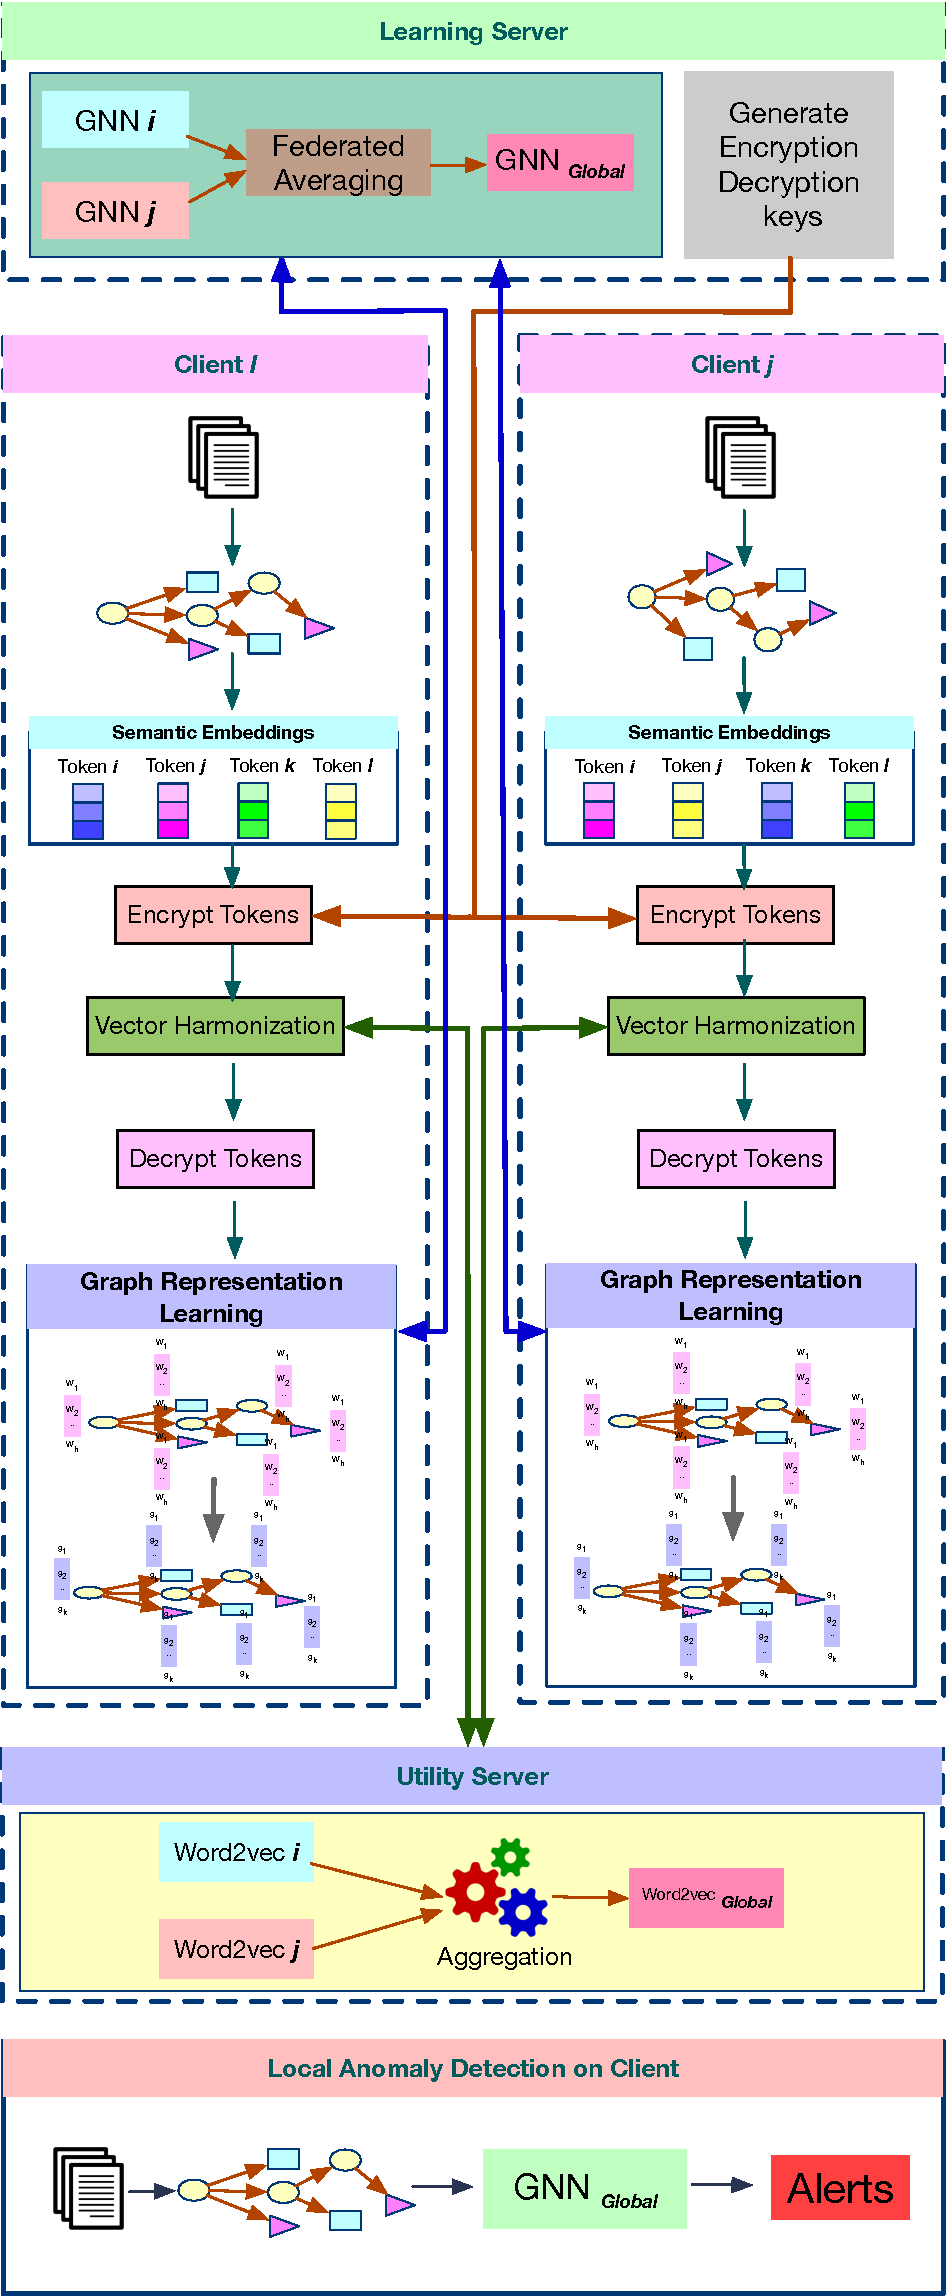
\includegraphics[width=0.45\textwidth]{fig/arch.pdf}
    \caption{High Level Architecture of \Sys}
    \vspace{-3ex}
    \label{arch}
  \end{figure}
